\documentclass[a4paper]{article}

%% Language and font encodings
\usepackage[english]{babel}
\usepackage[utf8x]{inputenc}
\usepackage[T1]{fontenc}

%% Sets page size and margins
\usepackage[a4paper,top=3cm,bottom=2cm,left=3cm,right=3cm,marginparwidth=2cm]{geometry}

%% Useful packages
\usepackage{amsmath}
\usepackage{amsfonts}
\usepackage{bbm}
\usepackage{graphicx}
\usepackage[colorinlistoftodos]{todonotes}
\usepackage[colorlinks=true, allcolors=blue]{hyperref}
\usepackage{float}
\usepackage{enumerate}
\usepackage{mathrsfs}
\usepackage{caption}
\usepackage{subcaption}

\usepackage{pgfplots, pgfplotstable}
\pgfplotsset{compat=1.16}
\pgfplotsset{soldot/.style={color=blue,only marks,mark=*}} \pgfplotsset{holdot/.style={color=blue,fill=white,only marks,mark=*}}

\title{Stochastic Processes}
\author{Kevin Chang}

\graphicspath{ {./image/} }

\begin{document}
\maketitle

\section{}
\begin{itemize}
        \begin{figure} [H]
            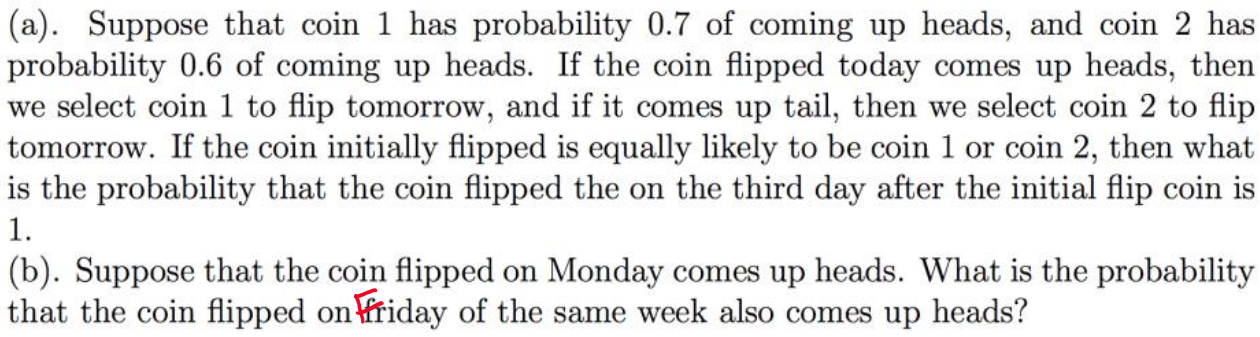
\includegraphics[width=1\linewidth]{image/1.png}
        \end{figure}
    \item $P = \left[ \begin{array}{cc} 0.7 & 0.3 \\ 0.6 & 0.4 \end{array} \right]$
    \item (a) $[0.5$ $0.5] P^3 = [0.6665$ $0.3335]$
    \item (b) $[1$ $0] P^3 = [0.6667$ $0.3333]$
\end{itemize}

\section{}
\begin{itemize}
        \begin{figure} [H]
            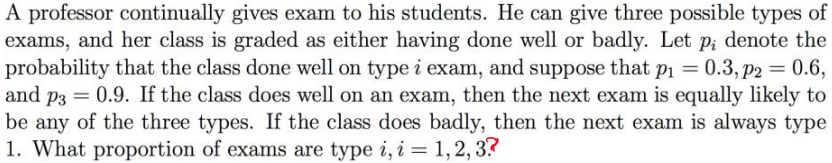
\includegraphics[width=1\linewidth]{image/2.png}
        \end{figure}
    \item $P = \left[ \begin{array}{ccc}
                0.8 & 0.1 & 0.1 \\
                0.6 & 0.2 & 0.2 \\
                0.4 & 0.3 & 0.3 \\
            \end{array} \right]$
    \item stationary distribution: $p$
        \begin{itemize}
            \item $p$ is eigenvector corresponding to eigenvalue 1 of $P^T$
            \item $p = [\frac{5}{7}$ $\frac{1}{7}$ $\frac{1}{7}]$
        \end{itemize}
\end{itemize}

\section{}
\begin{itemize}
        \begin{figure} [H]
            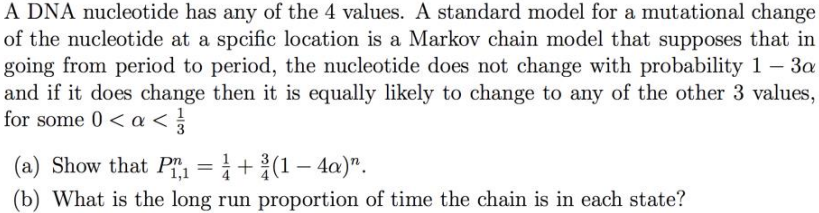
\includegraphics[width=1\linewidth]{image/3.png}
        \end{figure}
    \item $P = \left[ \begin{array}{cccc}
                1-3 \alpha & \alpha & \alpha & \alpha \\
                \alpha & 1-3 \alpha & \alpha & \alpha \\
                \alpha & \alpha & 1-3 \alpha & \alpha \\
                \alpha & \alpha & \alpha & 1-3 \alpha \\
            \end{array} \right]$
    \item (a)
        \begin{itemize}
            \item $P^n = \frac{1}{4}\left[ \begin{array}{cccc}
                        3(1-4\alpha)^n + 1 & 1 - (1-4\alpha)^n & 1 - (1-4\alpha)^n & 1 - (1-4\alpha)^n \\
                        1 - (1-4\alpha)^n & 3(1-4\alpha)^n + 1 & 1 - (1-4\alpha)^n & 1 - (1-4\alpha)^n \\
                        1 - (1-4\alpha)^n & 1 - (1-4\alpha)^n & 3(1-4\alpha)^n + 1 & 1 - (1-4\alpha)^n \\
                        1 - (1-4\alpha)^n & 1 - (1-4\alpha)^n & 1 - (1-4\alpha)^n & 3(1-4\alpha)^n + 1 \\
                \end{array} \right]$

                (by Wolfram Alpha)
            \item $P_{1, 1}^n = \frac{1}{4} + \frac{3}{4}(1-4\alpha)^n$
        \end{itemize}
    \item (b) it is equally distributed: stationary distribution is $\frac{1}{4}[1, 1, 1, 1]$
\end{itemize}

\section{}
\begin{itemize}
        \begin{figure} [H]
            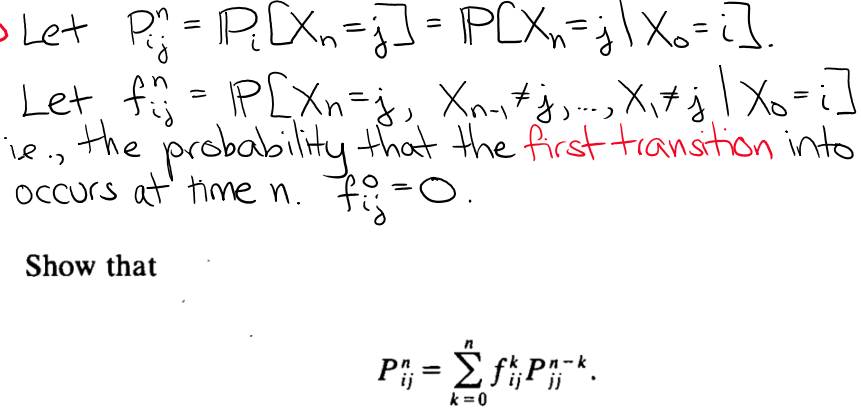
\includegraphics[width=1\linewidth]{image/4.png}
        \end{figure}
    \item $P_{ij}^n = P[X_n = j|X_0 = i] = P[X_n = j, X_1 = j|X_0=i] + P[X_n = j, X_1 \not = j|X_0=i]$

        $= P[X_n = j|X_1 = j, X_0=i]P[X_1=j|X_0=i] + P[X_n = j, X_1 \not = j|X_0=i]$

        $= P_{jj}^{n-1} f_{ij}^k + P[X_n = j, X_2 = j, X_1 \not = j|X_0=i] + P[X_n = j, X_2 \not = j, X_1 \not = j|X_0=i]$

        $= P_{jj}^{n-1} f_{ij}^2 + P_{jj}^{n-2} f_{ij}^2 + P[X_n = j, X_2 \not = j, X_1 \not = j|X_0=i]$

        $\dots$

        $= \sum_{k=0}^n P_{jj}^{n-k} f_{ij}^k$
\end{itemize}

\section{}
\begin{itemize}
        \begin{figure} [H]
            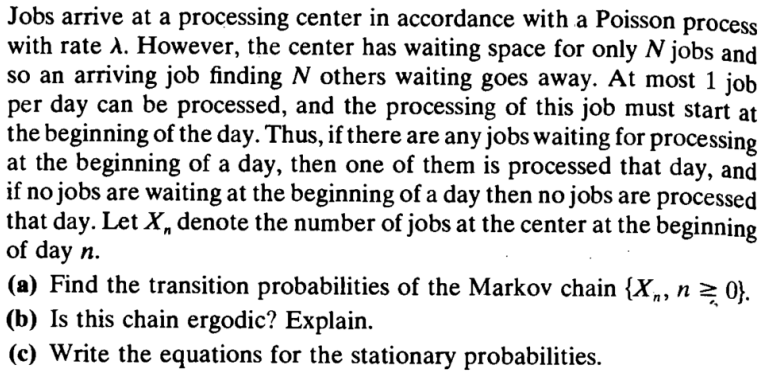
\includegraphics[width=1\linewidth]{image/5.png}
        \end{figure}
    \item 
\end{itemize}
\end{document}
